\documentclass[12pt,a4paper]{article}
\usepackage[utf8]{vietnam}
\usepackage{amsmath,amssymb}
\usepackage{tabularx}
\usepackage{tikz}
\usetikzlibrary{calc,angles,quotes,arrows.meta}
\usepackage{xcolor}
\usepackage{enumitem}
\usepackage{fancyhdr}
\usepackage[top=1.2cm, bottom=1.2cm, left=1.5cm, right=1.5cm]{geometry}
\usepackage[loigiai]{ex_test}

\setlength{\headheight}{15pt}
\setlength{\parskip}{0pt}

\pagestyle{fancy}
\fancyhf{}
\rhead{\textit{Môn Toán 7 -- Lời giải Đề số 4}}
\lhead{\textit{Bộ đề ôn tập Giữa học kì I}}
\cfoot{\thepage}

\begin{document}

\begin{center}
\textbf{\Large ĐÁP ÁN VÀ LỜI GIẢI CHI TIẾT -- ĐỀ SỐ 4}\\
\textit{Môn: TOÁN 7 -- Thời gian làm bài: 90 phút}
\end{center}
\vspace{2mm}

\noindent\textbf{\large PHẦN I. CÂU TRẮC NGHIỆM NHIỀU PHƯƠNG ÁN LỰA CHỌN}

\vspace{1mm}
\begin{ex}
Chọn câu trả lời đúng: Trong định lí: ``Nếu một đường thẳng vuông góc với một trong hai đường thẳng song song thì nó cũng vuông góc với đường thẳng kia''. Ta có giả thiết là:
\choice
{``Nếu một đường thẳng vuông góc''}
{``Nó cũng vuông góc với đường thẳng kia''}
{``Nếu một đường thẳng vuông góc với một trong hai đường thẳng song song thì nó cũng vuông góc với đường thẳng kia''}
{\True ``Một đường thẳng vuông góc với một trong hai đường thẳng song song''}
\loigiai{
Định lí toán học có dạng ``Nếu $A$ thì $B$'', trong đó phần nằm sau từ ``Nếu'' ($A$) là giả thiết, phần nằm sau từ ``thì'' ($B$) là kết luận. Mệnh đề sau từ ``Nếu'' là: ``Một đường thẳng vuông góc với một trong hai đường thẳng song song''.
}
\end{ex}

\begin{ex}
Số nào là số vô tỉ?
\choice
{$3{,}2$}
{$5{,}3(2)$}
{$0{,}6$}
{\True $-1{,}23427232\dots$}
\loigiai{
$3{,}2$ và $0{,}6$ là các số thập phân hữu hạn (số hữu tỉ). $5{,}3(2)$ là số thập phân vô hạn tuần hoàn (số hữu tỉ). $-1{,}23427232\dots$ là số thập phân vô hạn không tuần hoàn nên là số vô tỉ.
}
\end{ex}

\begin{ex}
Số đối của số hữu tỉ $-0{,}25$ là:
\choice
{$-0{,}25$}
{$-\dfrac{1}{4}$}
{$-4$}
{\True $0{,}25$}
\loigiai{
Số đối của số hữu tỉ $x$ là $-x$. Do đó, số đối của $-0{,}25$ là $-(-0{,}25) = 0{,}25$.
}
\end{ex}

\begin{ex}
Qua một điểm ở ngoài đường thẳng, ta kẻ được bao nhiêu đường thẳng song song với đường thẳng đó?
\choice
{$0$}
{\True $1$}
{$2$}
{$3$}
\loigiai{
Theo tiên đề Euclid, qua một điểm nằm ngoài một đường thẳng chỉ có duy nhất 1 đường thẳng song song với đường thẳng đó.
}
\end{ex}

\begin{ex}
Kết quả của phép tính $2^2 \cdot 2^5$ là:
\choice
{$2^{10}$}
{$2^3$}
{$2^5$}
{\True $2^7$}
\loigiai{
Áp dụng quy tắc nhân hai lũy thừa cùng cơ số: $2^2 \cdot 2^5 = 2^{2+5} = 2^7$.
}
\end{ex}

\begin{ex}
Cho hai số hữu tỉ $a$ và $b$ được biểu diễn trên trục số như sau. Chọn khẳng định đúng:
\begin{center}
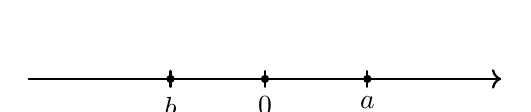
\begin{tikzpicture}[scale=1, line cap=round, line join=round]
  \draw[->, thick] (-3,0) -- (3,0);
  \draw[thick] (-1.2, -0.1) -- (-1.2, 0.1);
  \fill (-1.2, 0) circle (1.5pt);
  \node[below=3pt] at (-1.2, 0) {$b$};

  \draw[thick] (0, -0.1) -- (0, 0.1);
  \fill (0, 0) circle (1.5pt);
  \node[below=3pt] at (0, 0) {$0$};

  \draw[thick] (1.3, -0.1) -- (1.3, 0.1);
  \fill (1.3, 0) circle (1.5pt);
  \node[below=3pt] at (1.3, 0) {$a$};
\end{tikzpicture}
\end{center}
\choice
{$b > a > 0$}
{$b > a$}
{$b < a < 0$}
{\True $b < 0 < a$}
\loigiai{
Trên trục số nằm ngang, các số nhỏ hơn nằm ở bên trái, các số lớn hơn nằm ở bên phải. Do điểm $b$ nằm bên trái điểm $0$ và điểm $0$ nằm bên trái điểm $a$, ta có: $b < 0 < a$.
}
\end{ex}

\begin{ex}
\immini{
Tia phân giác của $\widehat{xOm}$ và $\widehat{yOn}$ lần lượt là:
\choice
{\True $Ok$ và $Ou$}
{$Ox$ và $Oy$}
{$Ou$ và $Om$}
{$Ok$ và $On$}
}{
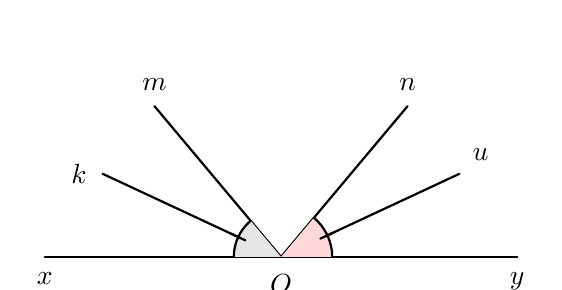
\begin{tikzpicture}[scale=1, line cap=round, line join=round]
  \coordinate (O) at (0,0);
  \draw[thick] (-3,0) node[below=2pt] {$x$} -- (3,0) node[below=2pt] {$y$};
  \draw[thick] (O) -- (130:2.5) node[above=2pt] {$m$};
  \draw[thick] (O) -- (155:2.5) node[left=2pt] {$k$};
  \draw[thick] (O) -- (50:2.5) node[above=2pt] {$n$};
  \draw[thick] (O) -- (25:2.5) node[above right=1pt] {$u$};

  \fill[gray!20] (O) -- (180:0.6) arc (180:130:0.6) -- cycle;
  \draw[thick] (180:0.6) arc (180:130:0.6);
  \draw[thick] (155:0.5) -- (155:0.7);

  \fill[red!15] (O) -- (0:0.65) arc (0:50:0.65) -- cycle;
  \draw[thick] (0:0.65) arc (0:50:0.65);
  \draw[thick] (25:0.55) -- (25:0.75);

  \node[below=3pt] at (O) {$O$};
\end{tikzpicture}
}
\loigiai{
Tia $Ok$ nằm giữa hai tia $Ox, Om$ và tạo thành hai góc bằng nhau nên $Ok$ là tia phân giác của $\widehat{xOm}$. Tia $Ou$ nằm giữa hai tia $Oy, On$ và tạo thành hai góc bằng nhau nên $Ou$ là tia phân giác của $\widehat{yOn}$.
}
\end{ex}

\begin{ex}
Cho một hình lăng trụ đứng có diện tích đáy là $S$, chiều cao là $h$. Công thức tính thể tích của hình lăng trụ đứng là:
\choice
{\True $V = S \cdot h$}
{$V = \dfrac{1}{2} S \cdot h$}
{$V = 2 S \cdot h$}
{$V = 3 S \cdot h$}
\loigiai{
Thể tích của hình lăng trụ đứng bằng diện tích đáy nhân với chiều cao: $V = S \cdot h$.
}
\end{ex}

\begin{ex}
Tính $\left[ \left(\dfrac{1}{3}\right)^2 \right]^4$ ta được:
\choice
{$\left(\dfrac{1}{3}\right)^2$}
{\True $\left(\dfrac{1}{3}\right)^8$}
{$\left(\dfrac{1}{3}\right)^6$}
{$\left(\dfrac{1}{3}\right)^4$}
\loigiai{
Áp dụng công thức lũy thừa của lũy thừa $(a^m)^n = a^{m \cdot n}$, ta có: $\left[ \left(\dfrac{1}{3}\right)^2 \right]^4 = \left(\dfrac{1}{3}\right)^{2 \cdot 4} = \left(\dfrac{1}{3}\right)^8$.
}
\end{ex}

\begin{ex}
Có bao nhiêu giá trị của $x \in \mathbb{Q}; x \ge 1$ sao cho $x^4 - x = 0$?
\choice
{\True $1$}
{$0$}
{$2$}
{$3$}
\loigiai{
Ta có: $x^4 - x = 0 \Leftrightarrow x(x^3 - 1) = 0 \Leftrightarrow x = 0$ hoặc $x^3 = 1 \Leftrightarrow x = 1$. Vì điều kiện $x \ge 1$ nên ta chỉ nhận $x = 1$. Vậy có duy nhất $1$ giá trị của $x$ thỏa mãn.
}
\end{ex}

\begin{ex}
\immini{
Cho hình vẽ sau, biết $Ob$ là tia phân giác của $\widehat{aOc}$. Khẳng định nào sau đây đúng?
\choice
{$\widehat{bOc} = 90^\circ$}
{\True $\widehat{bOc} = 60^\circ$}
{$\widehat{bOc} = 30^\circ$}
{$\widehat{bOc} = 120^\circ$}
}{
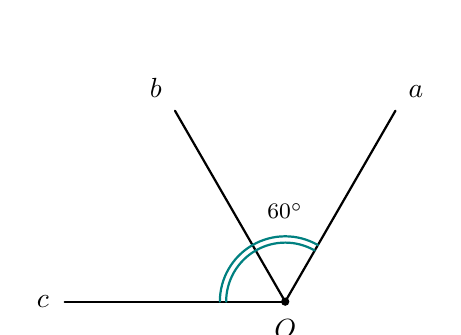
\begin{tikzpicture}[scale=1, line cap=round, line join=round]
  \coordinate (O) at (0,0);
  \draw[thick] (O) -- (-2.8,0) node[left=2pt] {$c$};
  \draw[thick] (O) -- (120:2.8) node[above left=1pt] {$b$};
  \draw[thick] (O) -- (60:2.8) node[above right=1pt] {$a$};

  \fill (O) circle (1.5pt) node[below=3pt] {$O$};

  \draw[teal, thick] (60:0.75) arc (60:120:0.75);
  \draw[teal, thick] (60:0.83) arc (60:120:0.83);
  \node[font=\footnotesize] at (90:1.15) {$60^\circ$};

  \draw[teal, thick] (120:0.75) arc (120:180:0.75);
  \draw[teal, thick] (120:0.83) arc (120:180:0.83);
\end{tikzpicture}
}
\loigiai{
Vì $Ob$ là tia phân giác của $\widehat{aOc}$ nên $\widehat{bOc} = \widehat{aOb}$. Quan sát hình vẽ ta có $\widehat{aOb} = 60^\circ$, suy ra $\widehat{bOc} = 60^\circ$.
}
\end{ex}

\begin{ex}
Trong các số sau, số nào là số vô tỉ?
\choice
{$-5$}
{$5{,}7$}
{\True $\sqrt{7}$}
{$\dfrac{5}{3}$}
\loigiai{
$-5$ là số nguyên (số hữu tỉ); $5{,}7 = \dfrac{57}{10}$ (số hữu tỉ); $\dfrac{5}{3}$ (số hữu tỉ). $\sqrt{7}$ là căn bậc hai số học của số không chính phương nên là số vô tỉ.
}
\end{ex}


\setcounter{ex}{0}
\noindent\textbf{\large PHẦN II. CÂU TRẮC NGHIỆM ĐÚNG SAI}

\vspace{1mm}
\begin{ex}
Cho $a, b, c, d \in \mathbb{Q}$. Xét tính đúng sai của các mệnh đề sau:
\choiceTF
{\True Bỏ dấu ngoặc của biểu thức $-(a + b - c)$ ta được kết quả $-a - b + c$}
{Bỏ dấu ngoặc của biểu thức $a + (-b - c + d)$ ta được kết quả $a - b - c - d$}
{Cho $a + b = c$, áp dụng quy tắc chuyển vế ta được $a = -b - c$}
{\True Cho $a - \dfrac{3}{4} = 5$, áp dụng quy tắc chuyển vế ta được $a = 5 + \dfrac{3}{4}$}
\loigiai{
\begin{itemize}[leftmargin=0.5cm, itemsep=1pt]
\item \textbf{a)} \textbf{Đúng}. Khi bỏ dấu ngoặc có dấu trừ ``$-$'' đằng trước, ta đổi dấu tất cả các số hạng trong ngoặc: $-(a + b - c) = -a - b + c$.
\item \textbf{b)} \textbf{Sai}. Khi bỏ dấu ngoặc có dấu cộng ``$+$'' đằng trước, ta giữ nguyên dấu các số hạng trong ngoặc: $a + (-b - c + d) = a - b - c + d \neq a - b - c - d$.
\item \textbf{c)} \textbf{Sai}. Chuyển số hạng $b$ từ vế trái sang vế phải ta đổi dấu thành $-b$, kết quả đúng phải là $a = c - b$.
\item \textbf{d)} \textbf{Đúng}. Chuyển số hạng $-\dfrac{3}{4}$ sang vế phải ta đổi dấu thành $+\dfrac{3}{4}$, kết quả là $a = 5 + \dfrac{3}{4}$.
\end{itemize}
}
\end{ex}

\begin{ex}
\immini{
Quan sát hình vẽ, hai đường thẳng $a$ và $b$ cắt nhau tại điểm $O$ tạo thành bốn góc $\widehat{O}_1, \widehat{O}_2, \widehat{O}_3, \widehat{O}_4$. Xét tính đúng sai của các mệnh đề sau:
\choiceTF
{\True Góc $\widehat{O}_1$ và góc $\widehat{O}_3$ là hai góc đối đỉnh}
{Góc $\widehat{O}_2$ và góc $\widehat{O}_4$ là hai góc kề bù}
{\True Tổng số đo của góc $\widehat{O}_1$ và góc $\widehat{O}_2$ bằng $180^\circ$}
{\True Nếu số đo góc $\widehat{O}_1$ bằng $60^\circ$ thì số đo góc $\widehat{O}_4$ bằng $120^\circ$}
}{
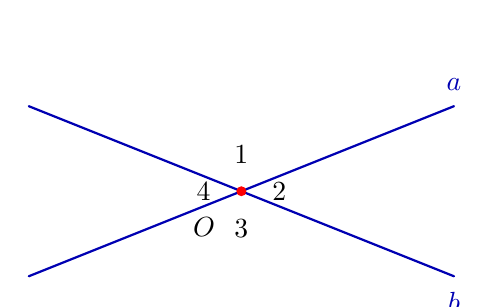
\begin{tikzpicture}[scale=0.9, line cap=round, line join=round]
  \coordinate (O) at (0,0);
  \draw[thick, blue!70!black] (-3,-1.2) -- (3,1.2) node[above=2pt] {$a$};
  \draw[thick, blue!70!black] (-3,1.2) -- (3,-1.2) node[below=2pt] {$b$};

  \fill[red] (O) circle (2pt);

  \node[above=2pt] at (0,0.18) {$1$};
  \node[right=2pt] at (0.22,0) {$2$};
  \node[below=2pt] at (0,-0.18) {$3$};
  \node[left=2pt] at (-0.22,0) {$4$};

  \node[below left=6pt] at (O) {$O$};
\end{tikzpicture}
}
\loigiai{
\begin{itemize}[leftmargin=0.5cm, itemsep=1pt]
\item \textbf{a)} \textbf{Đúng}. Hai góc $\widehat{O}_1$ và $\widehat{O}_3$ đối diện nhau qua đỉnh $O$, mỗi cạnh của góc này là tia đối của một cạnh góc kia nên là hai góc đối đỉnh.
\item \textbf{b)} \textbf{Sai}. Góc $\widehat{O}_2$ và góc $\widehat{O}_4$ là hai góc đối đỉnh, không phải hai góc kề bù.
\item \textbf{c)} \textbf{Đúng}. Góc $\widehat{O}_1$ và góc $\widehat{O}_2$ là hai góc kề bù nên tổng số đo của chúng bằng $180^\circ$.
\item \textbf{d)} \textbf{Đúng}. Do góc $\widehat{O}_1$ và góc $\widehat{O}_4$ là hai góc kề bù nên $\widehat{O}_4 = 180^\circ - \widehat{O}_1 = 180^\circ - 60^\circ = 120^\circ$.
\end{itemize}
}
\end{ex}


\setcounter{ex}{0}
\noindent\textbf{\large PHẦN III. CÂU HỎI TRẢ LỜI NGẮN}

\vspace{1mm}
\begin{ex}
Tính hợp lý giá trị của biểu thức: $A = \dfrac{-5}{9} \cdot \dfrac{4}{13} + \dfrac{-5}{9} \cdot \dfrac{9}{13} + \dfrac{5}{9}$. \shortans{$0$}
\loigiai{
Ta có:
\begin{align*}
A &= \dfrac{-5}{9} \left( \dfrac{4}{13} + \dfrac{9}{13} \right) + \dfrac{5}{9} \\
&= \dfrac{-5}{9} \cdot 1 + \dfrac{5}{9} = \dfrac{-5}{9} + \dfrac{5}{9} = 0.
\end{align*}
Đáp án: $0$.
}
\end{ex}

\begin{ex}
Cho hai góc kề bù $\widehat{AOB}$ và $\widehat{BOC}$, biết $\widehat{AOB} = 110^\circ$. Gọi $OM$ là tia phân giác của $\widehat{AOB}$. Tính số đo góc $\widehat{BOC}$ và $\widehat{COM}$. \shortans{$\widehat{BOC} = 70^\circ; \widehat{COM} = 125^\circ$}
\loigiai{
Vì $\widehat{AOB}$ và $\widehat{BOC}$ là hai góc kề bù nên:
\[ \widehat{BOC} = 180^\circ - \widehat{AOB} = 180^\circ - 110^\circ = 70^\circ. \]
Vì $OM$ là tia phân giác của $\widehat{AOB}$ nên:
\[ \widehat{BOM} = \dfrac{\widehat{AOB}}{2} = \dfrac{110^\circ}{2} = 55^\circ. \]
Vì tia $OB$ nằm giữa hai tia $OM$ và $OC$ nên:
\[ \widehat{COM} = \widehat{BOC} + \widehat{BOM} = 70^\circ + 55^\circ = 125^\circ. \]
Đáp án: $\widehat{BOC} = 70^\circ$ và $\widehat{COM} = 125^\circ$.
}
\end{ex}


\setcounter{ex}{0}
\noindent\textbf{\large PHẦN IV. TỰ LUẬN}

\vspace{1mm}
\begin{ex}
Thực hiện phép tính:
\begin{enumerate}[label=\textbf{\alph*)}, leftmargin=0.8cm, itemsep=1pt]
\item $\dfrac{5}{12} + \left(-\dfrac{7}{24}\right) : \dfrac{3}{8}$
\item $\left(-\dfrac{4}{5}\right) \cdot \dfrac{3}{7} - \dfrac{4}{7} : \sqrt{\dfrac{25}{16}} - |-1|$
\end{enumerate}
\loigiai{
\textbf{a)} Ta có:
\[ \dfrac{5}{12} + \left(-\dfrac{7}{24}\right) : \dfrac{3}{8} = \dfrac{5}{12} + \left(-\dfrac{7}{24}\right) \cdot \dfrac{8}{3} = \dfrac{5}{12} + \left(-\dfrac{7}{9}\right) = \dfrac{15 - 28}{36} = -\dfrac{13}{36}. \]

\textbf{b)} Ta có:
\begin{align*}
\left(-\dfrac{4}{5}\right) \cdot \dfrac{3}{7} - \dfrac{4}{7} : \dfrac{5}{4} - 1 &= -\dfrac{12}{35} - \dfrac{4}{7} \cdot \dfrac{4}{5} - 1 \\
&= -\dfrac{12}{35} - \dfrac{16}{35} - 1 \\
&= -\dfrac{28}{35} - 1 = -\dfrac{4}{5} - 1 = -\dfrac{9}{5}.
\end{align*}

}
\end{ex}
\vspace{1mm}

\begin{ex}
Tìm $x$ biết:
\begin{enumerate}[label=\textbf{\alph*)}, leftmargin=0.8cm, itemsep=1pt]
\item $\dfrac{3}{5} x + \dfrac{2}{3} = \dfrac{2^3}{3}$
\item $2 \sqrt{x} - 1 = 0$
\end{enumerate}
\loigiai{
\textbf{a)} Ta có:
\begin{align*}
\dfrac{3}{5} x + \dfrac{2}{3} &= \dfrac{8}{3} \\
\dfrac{3}{5} x &= \dfrac{8}{3} - \dfrac{2}{3} = \dfrac{6}{3} = 2 \\
x &= 2 : \dfrac{3}{5} = 2 \cdot \dfrac{5}{3} = \dfrac{10}{3}.
\end{align*}

\textbf{b)} Điều kiện: $x \ge 0$.
\[ 2 \sqrt{x} = 1 \Rightarrow \sqrt{x} = \dfrac{1}{2} \Rightarrow x = \left(\dfrac{1}{2}\right)^2 = \dfrac{1}{4} \text{ (thỏa mãn)}. \]

}
\end{ex}
\vspace{1mm}

\begin{ex}
Một siêu thị nhập vào 250 hộp bánh với giá bán niêm yết là 120 000 đồng/hộp. Đợt thứ nhất siêu thị bán được $\dfrac{3}{5}$ số hộp bánh với đúng giá niêm yết. Đợt thứ hai vì muốn kích cầu tiêu dùng, siêu thị đã giảm giá 8\% so với giá niêm yết ban đầu và đã bán hết số hộp bánh còn lại.
\begin{enumerate}[label=\textbf{\alph*)}, leftmargin=0.8cm, itemsep=1pt]
\item Hỏi đợt thứ nhất siêu thị đã bán được bao nhiêu hộp bánh và thu về được bao nhiêu tiền?
\item Cả hai đợt siêu thị đã thu về được bao nhiêu tiền?
\end{enumerate}
\loigiai{
\textbf{a)} Số hộp bánh bán được trong đợt thứ nhất là:
\[ 250 \cdot \dfrac{3}{5} = 150 \text{ (hộp)}. \]
Số tiền thu về trong đợt thứ nhất là:
\[ 150 \cdot 120\,000 = 18\,000\,000 \text{ (đồng)}. \]

\textbf{b)} Số hộp bánh bán trong đợt thứ hai là: $250 - 150 = 100$ (hộp).

Giá bán một hộp bánh ở đợt thứ hai sau khi giảm 8\% là:
\[ 120\,000 \cdot (100\% - 8\%) = 120\,000 \cdot 0{,}92 = 110\,400 \text{ (đồng)}. \]
Số tiền thu về trong đợt thứ hai là:
\[ 100 \cdot 110\,400 = 11\,040\,000 \text{ (đồng)}. \]
Tổng số tiền siêu thị thu về sau cả hai đợt là:
\[ 18\,000\,000 + 11\,040\,000 = 29\,040\,000 \text{ (đồng)}. \]

}
\end{ex}
\vspace{1mm}

\begin{ex}
\immini{
Cho tam giác $ABC$ có $BA = BC$. Gọi $M$ là trung điểm của đoạn thẳng $AC$. Chứng minh rằng: $\widehat{ABM} = \widehat{CBM}$.
}{
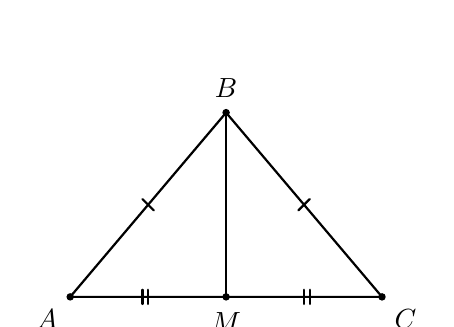
\begin{tikzpicture}[scale=0.9, line cap=round, line join=round]
  \coordinate (B) at (0,2.6);
  \coordinate (A) at (-2.2,0);
  \coordinate (C) at (2.2,0);
  \coordinate (M) at (0,0);

  \draw[thick] (A) -- (B) -- (C) -- cycle;
  \draw[thick] (B) -- (M);

  \fill (A) circle (1.5pt) node[below left=1pt] {$A$};
  \fill (B) circle (1.5pt) node[above=2pt] {$B$};
  \fill (C) circle (1.5pt) node[below right=1pt] {$C$};
  \fill (M) circle (1.5pt) node[below=2pt] {$M$};

  \draw[thick] ($(A)!0.5!(B)+(-0.08,0.08)$) -- ($(A)!0.5!(B)+(0.08,-0.08)$);
  \draw[thick] ($(C)!0.5!(B)+(-0.08,-0.08)$) -- ($(C)!0.5!(B)+(0.08,0.08)$);

  \draw[thick] (-1.1,-0.1) -- (-1.1,0.1);
  \draw[thick] (-1.18,-0.1) -- (-1.18,0.1);
  \draw[thick] (1.1,-0.1) -- (1.1,0.1);
  \draw[thick] (1.18,-0.1) -- (1.18,0.1);
\end{tikzpicture}
}
\loigiai{
Xét $\Delta ABM$ và $\Delta CBM$, ta có:
\[ \begin{aligned} BA &= BC \quad \text{(theo giả thiết)}, \\ AM &= MC \quad \text{(vì $M$ là trung điểm của $AC$)}, \\ BM &\quad \text{là cạnh chung}. \end{aligned} \]
Suy ra $\Delta ABM = \Delta CBM$ (c-c-c).

Do đó $\widehat{ABM} = \widehat{CBM}$ (hai góc tương ứng).
}
\end{ex}
\vspace{1mm}


\begin{center}
\rule{4cm}{0.4pt}\\
\textit{--- HẾT ---}
\end{center}
\end{document}
